\documentclass[11pt, oneside]{article}
\usepackage[utf8]{inputenc}                        % utf8
\usepackage[T1]{fontenc}                           % fix font encoding
\usepackage[english]{babel}                        % language
\usepackage{titling, geometry, hyperref, fancyhdr, algorithm}
\usepackage{amsmath, amssymb, amsthm}              % ams mathematical packages
\usepackage{physics, mathtools, bm}                % extra math packages
\usepackage{graphicx, subcaption, wrapfig}         % images
\usepackage{fvextra, textcomp, CJKutf8}            % misc. text formatting
\usepackage[autostyle, english=american]{csquotes} % quotes
\usepackage[shortlabels]{enumitem}                 % lists
\usepackage{tikz, pgfplots, tikz-network}          % plots and graphs
\usepackage[noend]{algpseudocode}                  % algorithm psuedocode
\usepackage[cache=true]{minted}                    % source code
\usepackage[style=ieee]{biblatex}                  % bibliography
\geometry{a4paper}

\pgfplotsset{compat=1.17}                          % version of pgfplots

\hypersetup{
  colorlinks=true,
  urlcolor=cyan,
  linkcolor=magenta
}

\setminted[]{
  linenos=false,
  breaklines=true,
  encoding=utf8,
  fontsize=\normalsize,
  frame=lines,
  framesep=2mm
}

% https://tex.stackexchange.com/questions/343494/minted-red-box-around-greek-characters
\makeatletter
\AtBeginEnvironment{minted}{\dontdofcolorbox}
\def\dontdofcolorbox{\renewcommand\fcolorbox[4][]{##4}}
\makeatother

\graphicspath{{./images/}}
\addbibresource{ref.bib}

\title{manGANime: Future Video Prediction \\ with Conditional GANs}
\author{Stephen Huan, Luke Thistlethwaite}
\date{Thomas Jefferson High School for Science and Technology \\
      Computer Systems Lab 2020--2021}

\begin{document}
% {\hypersetup{linkcolor=black}
% \tableofcontents
% }
\maketitle

\begin{abstract}
  Unsupervised image synthesis has made enormous progress recently, especially
  with a class of models called generative adversarial networks (GANs).
  However, work on video generation remains stagnant because of its inherent
  difficulty. We consider a simplified domain for video generation by
  generating cartoon video (\enquote{anime}), and create a novel dataset for
  this task. We are then able to generate videos in an autoregressive and
  self-supervised manner, conditioning GANs on previous video frames as well
  as the comic book (\enquote{manga}) pages which inspired the original anime.
  Source code is available here:
  \href{https://github.com/stephen-huan/manGANime}
       {https://github.com/stephen-huan/manGANime}.
\end{abstract}

\section{Introduction} \label{sec:intro} 
A class of neural networks called generative adversarial networks (GANs)
are now able to generate images of astounding quality and resolution.
StyleGAN is able to generate very realistic images of human faces at a
resolution of 1024x1024 \cite{stylegan}, the quality of which was later
improved in StyleGAN2 \cite{stylegan2}, and finally further developed to
use less data with an adaptive discriminator augmentation system, dubbed
StyleGAN2-ADA \cite{stylegan2ada}.

A natural extension of image generation is \emph{video} generation, to generate
multiple images in a coherent sequence. There are varying formulations of video
generation, but we will consider the specific problem of \emph{future video
prediction}: given a few initial conditioning frames, predict the frames that
follow. This provides more structure compared to completely unsupervised video
generation, since the model is provided with conditioning frames and therefore
\enquote{has something to go off of}. Another benefit is that a model could be
trained with pure self-supervision, since the ground truth video is known.

However, the aforementioned successes in unsupervised \emph{image}
generation have not necessarily translated to \emph{video} generation.
The current state of the art in future video prediction is comparatively
limited; \enquote{\ldots there has been relatively little work extensively
studying generative adversarial networks for video} \cite{scene}. In
particular, the DVD-GAN model generates up to 48 frames (4 seconds) at a
resolution of 256x256 \cite{dvdgan}, a much smaller resolution and for
a duration too short for most content generation applications.

Motivated by these shortcomings, we propose a simplified domain for
video generation which will naturally improve results due to the
abstractions inherent to this domain. StyleGAN and DVD-GAN are both
most frequently trained on real-world datasets, for example the FFHQ
dataset of human faces and the Kinetics-600 dataset of YouTube videos
of human actions \cite{stylegan, dvdgan}. We propose instead applying
video generation algorithms to cartoon video, specifically a subset
of animations produced in Japan called \emph{anime}.

Our reasons for focusing on anime are as follows: first, there is a large
volume of unlabeled anime on the internet. A popular online anime steaming
service, Crunchyroll, has over 800 shows in its catalog \cite{crunchyroll},
which assuming an average of around 12 episodes per show and 20 minutes per
episode, corresponds to over 3,000 hours of video. The variance in visual
style is also lower than that of American animation, for example. Secondly,
many assumptions existing algorithms make are justified in anime. DVD-GAN,
for example, skips every other frame as it can \enquote{\ldots generate
videos with more complexity without incurring higher computational cost}
\cite{dvdgan}. Correspondingly, anime is often animated \enquote{on twos}, with
every other frame duplicated, or even on threes or fours. \cite{wikipedia}.
\citeauthor*{scene} \cite{scene} use convolutional GANs to model a dynamic
foreground separately from a static background, masking them into a final
video. Again, anime is actually created with an explicit foreground/background
separation, as shown by specialized companies dedicated to producing background
animation \cite{kusanagi}. Thus, while the real world thwarts assumptions,
anime is known to obey these priors \textit{a priori}. Finally, there is a
huge demand for anime, as shown by Crunchyroll's over 20 million users and 1
million paid subscribers \cite{crunchyroll}, but a shortage of labor causing
animators to work long hours for low pay \cite{vox}. Machine learning systems
like the ones already used by Sony \cite{deadline} can automate tedious work,
allowing animators to focus on the creative aspects of their work.

Note that anime is not so abstract as to destroy any semblance of the real
world, since algorithms on the real world apply to anime. For example,
the popular object detection model YOLOv4, trained on the MS COCO dataset
consisting of real world images \cite{yolov4} can be directly applied to
anime without transfer learning, as shown in \autoref{fig:object}.

\begin{figure}[h!]
  \centering
  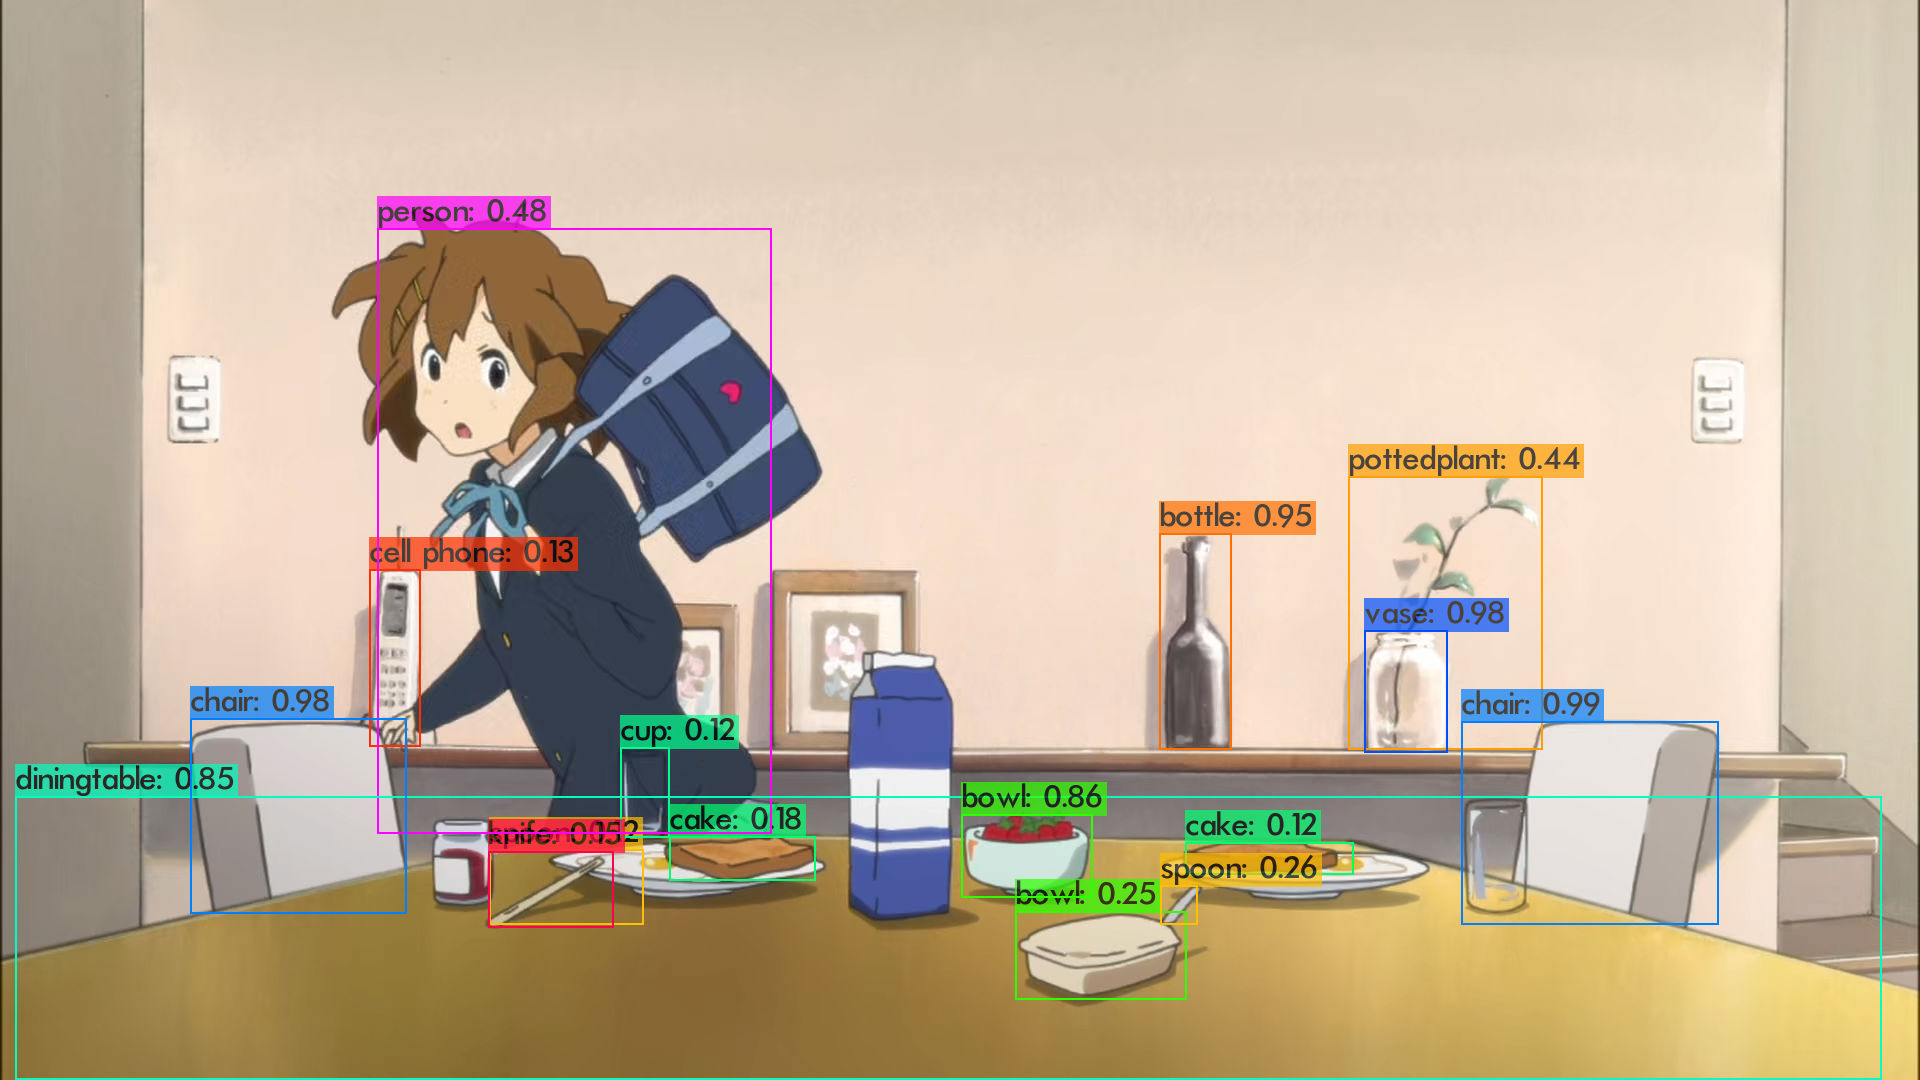
\includegraphics[scale=0.18,trim={0 0 0 190px},clip]{yolov4}
  \caption{The official implementation of YOLOv4-CSP \cite{yolov4}
    on an image from \textit{K-On!} \cite{kon!}, threshold of 0.1. See
    \href{https://youtu.be/i8jCzh9nWc4}{https://youtu.be/i8jCzh9nWc4}
    for a full demonstration.}
  \label{fig:object}
\end{figure}

In this paper, we show how to efficiently create a dataset of anime, each frame
of which is tagged with its corresponding comic book (\textit{manga}) page, a
useful conditioning signal justified in \autoref{sec:manga}. We create such a
dataset on \textit{Girls' Last Tour} \cite{tour}.

We then experiment with conditioning StyleGAN2-ADA \cite{stylegan2ada} on the
resulting dataset in order to generate video autoregressively, and with linear
interpolation in the latent space of the model to create smooth transitions
between two frames.

\section{Related Work}

\paragraph{Video generation}
Previous work on applying GANs to video generation include the aforementioned
\citeauthor*{scene} paper, which also makes use of large amounts of unlabeled
video, models the foreground separately from the background, and experiments
with adapting the discriminator for class prediction and the generator to
future video prediction with a simple conditioning scheme, encoding the
initial frame into the latent vector \cite{scene}. The current state of the
art model on the Kinetics-600 and UCF-101 datasets is the aforementioned Dual
Video Discriminator GAN (DVD-GAN), whose key insight is to have two (dual)
discriminators, one for measuring the realism of each frame and another for
measuring the realism of the video's motion as a whole; the separation of
concerns allows each discriminator to act more efficiently \cite{dvdgan}. We
deviate from these approaches in conditioning an image generator for video
generation rather than directly modeling videos as a 3D volume.
% smallest 568.942, largest 968.935, average of 720.587
We also condition upon manga, so the number of frames per manga page determines
our target length. Our dataset averages 360 frames per page, skipping every
other frame. DVD-GAN, however, generates only at most 48 frames \cite{dvdgan}.

\paragraph{Attention}
A technique that has proved very useful in language modeling is attention,
intuitively a set of weights guiding what the network pays attention to.
These weights are learned with gradient decent as usual. The landmark paper
\citetitle{attention} introduced the \emph{transformer} architecture, a model
which abandons the recurrent and convolutional connections popular in language
modeling in favor of pure attention, hence \enquote{Attention is All You Need}
\cite{attention}. \cite{transformer} then takes this transformer architecture
and applies it to video generation, attaining state of the art performance on
the BAIR robot pushing dataset with the resulting \emph{video transformer}.
We hypothesize that attention is a useful mechanism to guide a model's focus
on its conditioning information, especially if its conditioning signal is
as structured and sequence-like as manga. We do not, however, use standard
autoregressive modeling techniques like recurrent connections or attention, and
instead attempt to autoregressively generate video with conditioning alone.

\paragraph{Latent space exploration}
\citeauthor*{steer} experiment with \enquote{steering} GAN output by performing
walks in the latent space. Their learned walks perform modifications like color
changes, rotations, and camera zooms; they find that a linear walk performs as
well as a nonlinear walk \cite{steer}. We experiment with linear interpolation
in the latent space to generate transitions between two images, finding
that the resulting video is \enquote{smooth}, as would be expected from the
perceptual path regularization done by StyleGAN \cite{stylegan, stylegan2}.

\section{Dataset} \label{sec:manga}
Before discussing our methods for video generation, we first begin with
an analysis to efficiently construct an anime dataset tagged with manga.

\subsection{Picking an Anime} 
We make use of the large amounts of unlabeled video described in the
\hyperref[sec:intro]{introduction}. However, because we focus on applying
future video prediction to the domain of anime, we have an yet another
advantage that the real world doesn't: source material. Production of
anime is expensive, so anime is often animated with reference to a comic
book, or \textit{manga}. Certain anime will follow their source manga
very precisely, as shown in \autoref{fig:dual}.

\begin{figure}[h!]
    \centering
    \begin{subfigure}[h]{0.49 \textwidth}
      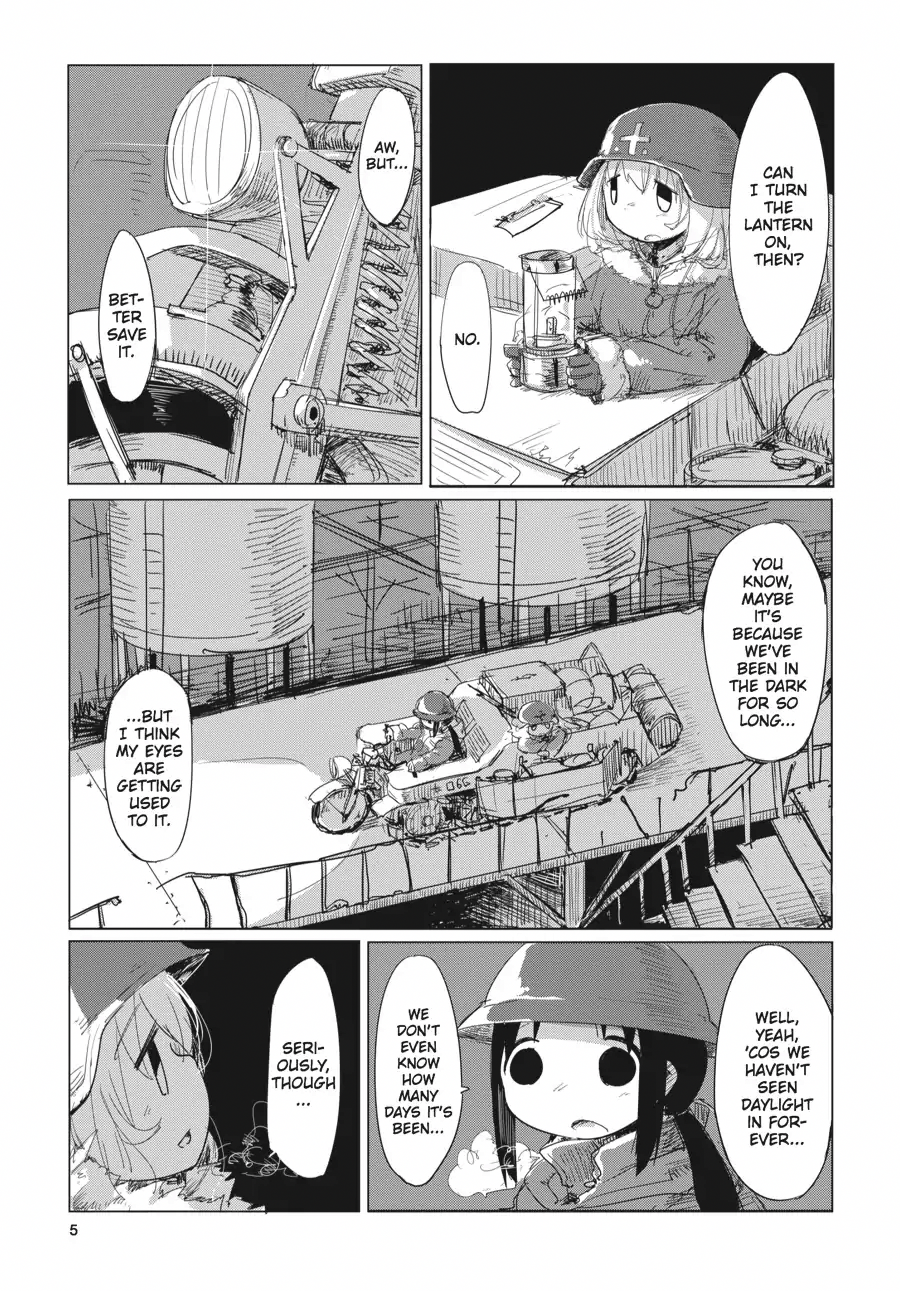
\includegraphics[scale=0.15,trim={60px 50px 60px 60px},clip]{page}
      \caption{A manga page from \textit{Girls' Last Tour}, \cite{tour1}.}
    \end{subfigure}
    \hfill
    \begin{subfigure}[h]{0.49 \textwidth}
      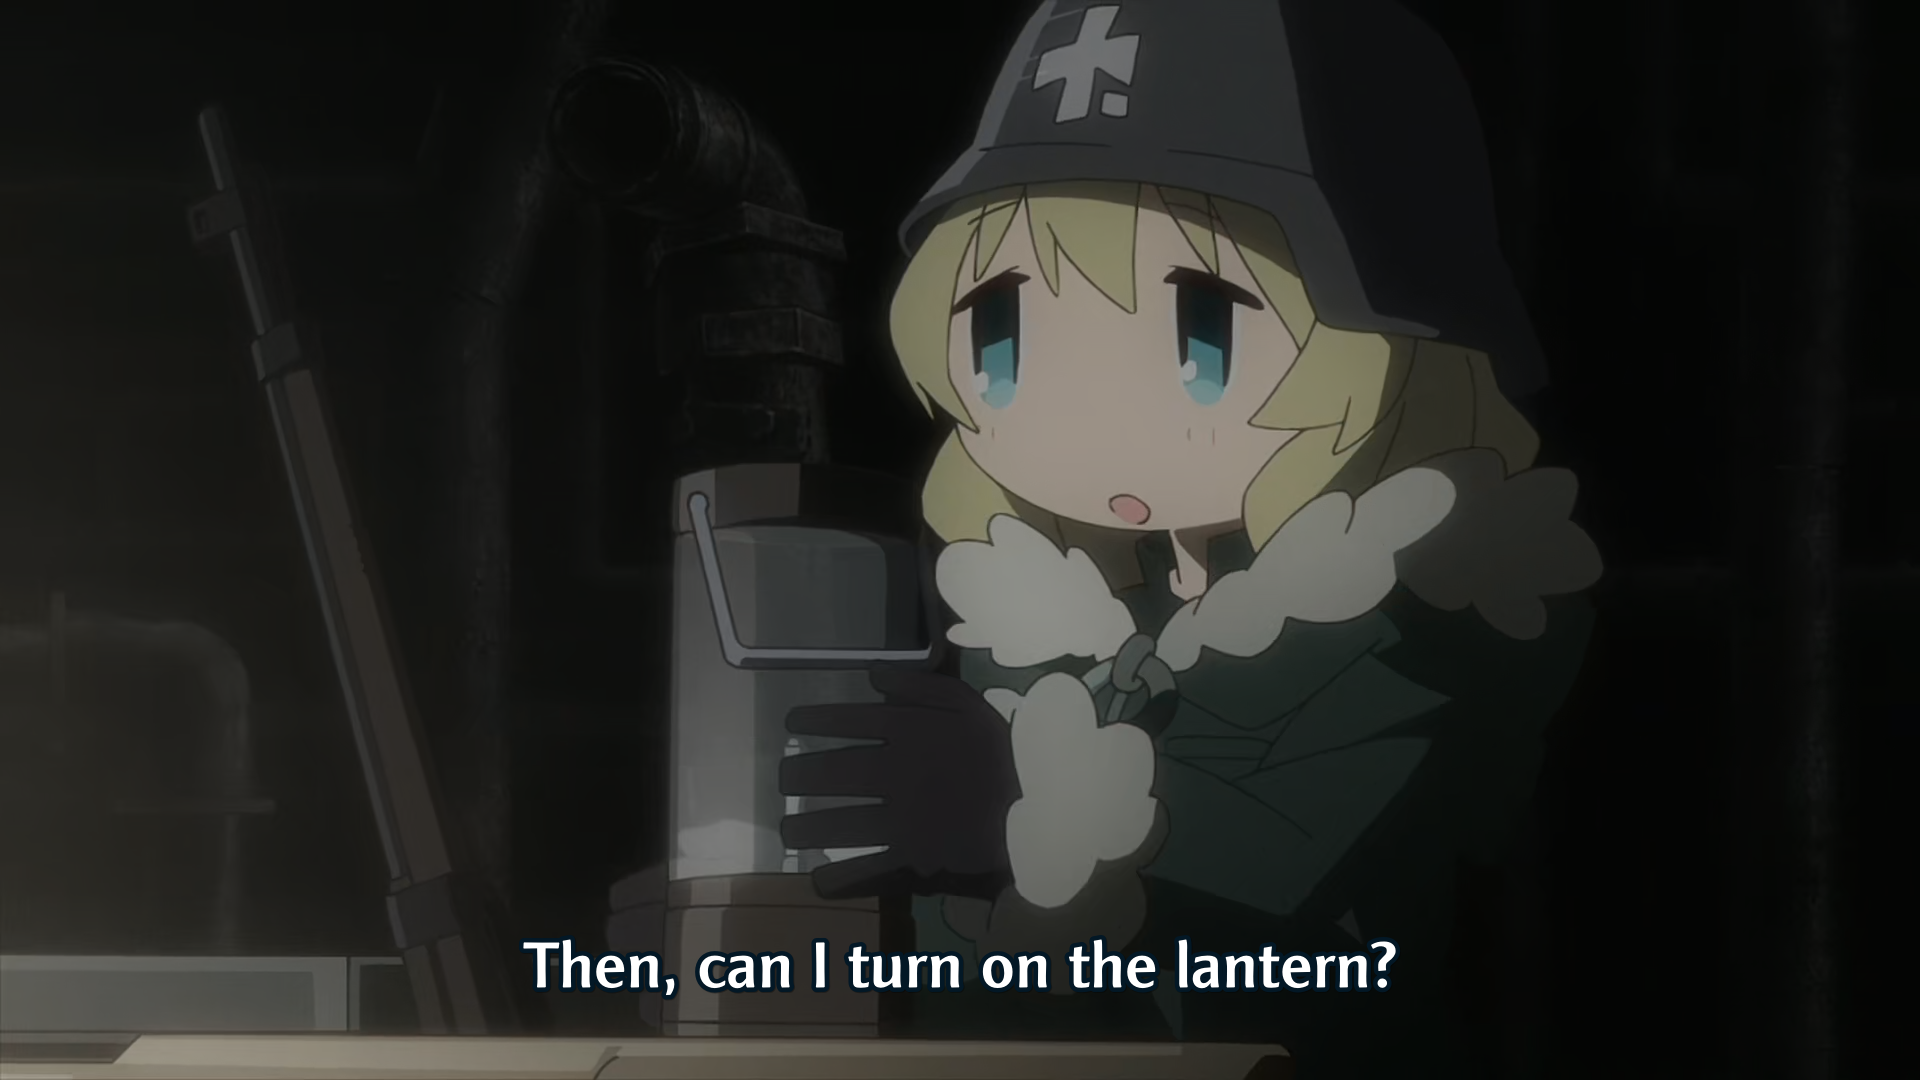
\includegraphics[scale=0.14,trim={180px 0 300px 0},clip]{frame}
      \caption{A anime frame from \textit{Girls' Last Tour}, \cite{tour}.}
    \end{subfigure} 
    \caption{The correspondence between anime and manga.}
    \label{fig:dual}
\end{figure}

It is useful, therefore, to find anime with a high correspondence with
its source manga. Formally speaking, we define a \textit{page function}
\( f: \mathbb{Z} \to \mathbb{Z} \) that maps an anime frame index to its
corresponding manga page. By the definition of a function, each element in
the domain must be mapped to an element in the co-domain. Since our domain
is anime frames, the existence of \( f \) implies that each anime frame
has a correspondence in manga. This means we will remove frames that have
no basis in manga, for example, the \enquote{intro} and \enquote{outro}
songs at the beginning/end of most episodes. We further enforce that \( f
\) is monotonic, i.e. \( x \leq y \) implies \( f(x) \leq f(y) \). This
implies the anime \enquote{goes in the same order} as the manga, which we
will see simplifies the construction of \( f \) immensely.

Many anime/manga pairs fulfill these conditions; we considered \textit{Girls'
Last Tour} \cite{tour} and its corresponding manga \cite{tour1, tour2, tour3,
tour4}, \textit{K-On!} \cite{kon!} and its second season \textit{K-On!!}
\cite{kon!!} and their corresponding manga \cite{kon1, kon2, kon3, kon4} among
others. We decided on \textit{Girls' Last Tour} because of its consistent
visual style and authors' familiarity with the material. The following analysis
will therefore use the quantitative features of \textit{Girls' Last Tour}.

\subsection{Exploiting Monotonicity for Efficient Tagging}
Suppose we have an anime/manga pair and wish to construct \( f \), that is,
to tag each frame of the anime with its corresponding manga page. Since the
average anime has 12 episodes, each episode is around 20 minutes without
intros/outros, and we sample at 12 FPS, skipping ever other frame, we will
have around 170,000 frames to process, exactly 174,792 total frames for
\textit{Girls' Last Tour} and 533 manga pages, which is too much to efficiently
label by hand. But because \( f \) is monotonic, we do not need to tag each
frame; we only need to tag the \textit{boundaries} when \( f \) changes.
For example, if we know \( f(0) = 2 \) and \( 600 \) is the smallest index
such that \( f(600) = 3 \), then that implies the frame indexes 1--599 must
be \( 2 \) by monotonicity. Thus, instead of tagging each frame one by one,
we can tag in batches determined by the transitions between manga pages,
reducing the number of operations from 170,000 (the number of anime frames) to
approximately 533 operations (the number of manga pages). This is implemented
in a graphical user interface (GUI) shown in \autoref{fig:tag}. However, we
still need to find which frames mark a transition between manga pages. Because
these critical frames naturally mark a transition in the anime as well, we
hypothesize they can be automatically detected by measuring similarity.

\begin{figure}[h!]
  \centering
  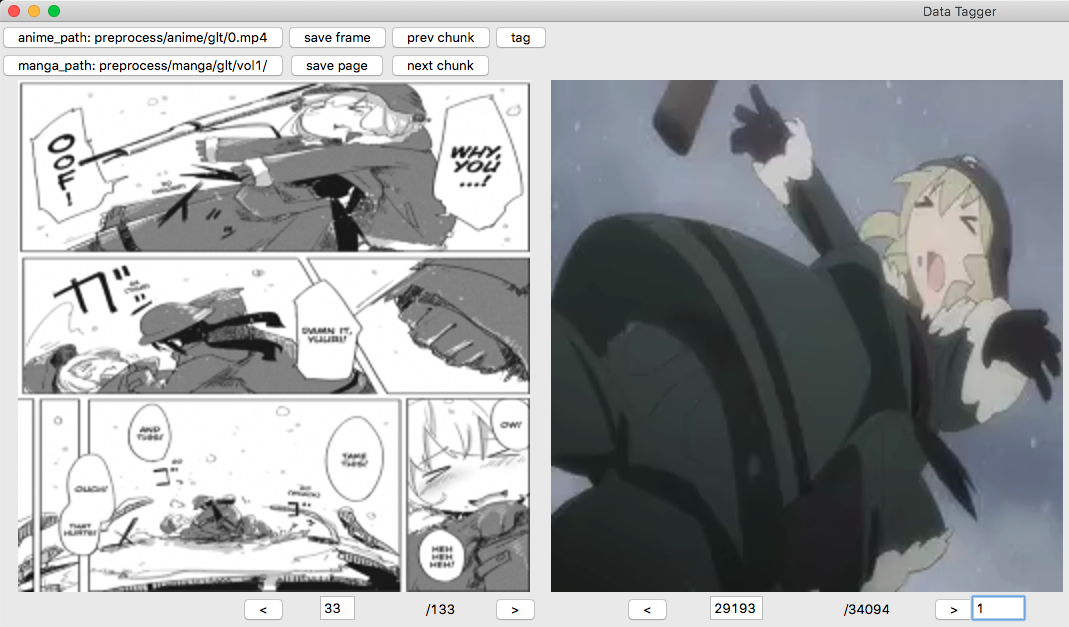
\includegraphics[scale=0.39]{data_tagger}
  \caption{Python \texttt{tkinter} GUI for efficient manual data
    tagging. The interface permits navigation with the left/right
    arrows as well as jumping to an arbitrary index. Pressing the
    \enquote{tag} button implicitly tags the frames up to the current
    frame. The \enquote{next chunk} button automatically moves to the
    next transition, determined by a low similarity between adjacent
    frames. \href{https://soft-matter.github.io/pims/v0.5/}{\texttt{pims}}
    is used for lazy loading of the underlying image data.}
  \label{fig:tag}
\end{figure}

\subsection{Measuring Frame Similarity}
We want to quantify a visual transition between two frames. We can do this by
computing a similarity metric between adjacent frames, and if it is lower than
a certain cutoff, declare that a transition must have happened between these
two frames. Two vectors are similar if they point in the same direction, which
can be measured with the \textit{cosine similarity}:
\[ \rho(\bm{u}, \bm{v}) = \cos{\alpha} = 
   \frac{\bm{u} \cdot \bm{v}}{\norm{\bm{u}} \norm{\bm{v}}} \]

This metric varies between -1 and 1, and a higher value implies greater
similarity. We intuitively generalize this dot product similarity to the
element-wise product of two tensors, which for two matrices \( A, B \)
can be written as follows:
\[ \begin{bmatrix} \bm{a}_1 & \bm{a}_2 & \dots & \bm{a}_n \end{bmatrix} \cdot
   \begin{bmatrix} \bm{b}_1 & \bm{b}_2 & \dots & \bm{b}_n \end{bmatrix}
   = \bm{a}_1 \cdot \bm{b}_1 + \bm{a}_2 \cdot \bm{b}_2 + \dots + \bm{a}_n \cdot \bm{b}_n
   = \sum^n_{i = 1} \sum^n_{j = 1} A_{ij} B_{ij} 
\]
Our similarity is then \( \rho(A, B) = \frac{A \cdot B}{\norm{A} \norm{B}} \)
where \( \norm{X} = \sqrt{X \cdot X} \) as usual.

For our particular anime, we found a cutoff of 0.8 worked well. If the user
presses the \enquote{next chunk} button in the GUI, \autoref{fig:tag}, then
the program computes the closest frame such that the similarity between
it and the next frame is less than 0.8. We naturally suffer from the
\textit{precision-recall trade-off}, since if the cutoff is higher we miss
transitions and if the cutoff is lower we encounter spurious transitions.
Future work may take into account more sophisticated measures of similarity,
for example, by measuring the difference in deep VGG16 embeddings which is
shown to align with human perception of similarity \cite{vgg}, or by taking
into account changes in optical flow \cite{flow}.

\subsection{Relative Number of Monotonic Functions}
Another approach to tagging data might be to train a neural network to
approximate the page function \( f \). Monotonicity still is helpful, as it
restricts the number of possible functions for \( f \). Suppose we have \( n \)
anime frames and \( k \) manga pages. If \( f \) was unconstrained, we'd have
\( n \) choices of \( k \) possibilities, \( k^n \) possibilities. However, \(
f \) is constrained to be monotonic. A function is monotonic if and only if its
outputs are sorted when read from increasing order of its inputs (this follows
from the definition of sorted being essentially identical to the definition of
a discrete monotonic function). A list has a unique sorted representation, so a
monotonic function is entirely determined by the \textit{values} of its outputs
and not the ordering. For example, if we want to find a monotonic function
from \( \{ 1, 2, 3 \} \) to \( \{ 4, 5, 6 \} \) and our output values are 4,
5, and 4, we must assign \( f(1) = 4 \), \( f(2) = 4 \), and \( f(3) = 5 \).
Thus, the number of monotonic functions from \( n \) values to \( k \) values
is the number of ways to put \( n \) unlabeled balls into \( k \) labeled
boxes. By the classic \enquote{stars and bars} argument, the number of ways is
\( {n + k - 1 \choose n} \). For \( n = 174792 \) and \( k = 533 \), there are
over \( 10^{1225} \) less monotonic functions than unconstrained functions, so
enforcing monotonicity drastically reduces the functional space.

\section{Methods}
\paragraph{Background}
A generative adversarial network (GAN) is composed of a generator \( G \) and
a discriminator \( D \) \cite{gans}. Intuitively, the generator attempts to
generate realistic output while the discriminator attempts to discern between
real and generated images \cite{gans}. Since the generator is trying to fool
the discriminator while the discriminator is trying to catch the generator,
the two are locked in competition, hence \enquote{adversarial networks}. In
order to allow the generator to generate varied output, a \textit{latent code}
or \textit{latent vector} \( \bm{z} \) is provided to the generator whose
elements are sampled i.i.d. from the standard normal distribution with mean
0 and standard deviation 1, \( \bm{z} \sim \mathcal{N}(0, 1) \).

The StyleGAN papers \cite{stylegan, stylegan2} modify this basic setup by
introducing a \textit{mapping network} \( f: \mathcal{Z} \to \mathcal{W}
\), which takes in a standard latent vector \( \bm{z} \) and produces \(
\bm{w} \in \mathcal{W} \). Intuitively, this mapping network allows \(
\bm{w} \) to be \enquote{disentangled} from the characteristics of the
training distribution, allowing for easier generation \cite{stylegan}.

\paragraph{StyleGAN}
We first directly train StyleGAN on our dataset, specifically StyleGAN2
with adaptive discriminator augmentation (ADA), an adaptation that allows
for better training on low volume datasets by automatically augmenting the
dataset with simple geometric transformations like rotations, translations,
and color changes \cite{stylegan2ada}.

\paragraph{Future Video Prediction}
With an unconditional model trained, we condition the model for future video
prediction similar to \cite{scene} by inserting image data into the latent
vector. Unlike \cite{scene}, we fully \textit{replace} the latent with our
image data. The dimensionality of the latent \( \bm{z} \) is 512 while we
need to fit two 256x256 images, so we greyscale both images and then apply a
16x16 average pool to reduce each image to \( 16^2 = 256 \) parameters, then
concatenate the two flattened images to form the vector \( \bm{x} \). Finally,
we transform \( \bm{x} \) into \( \bm{z} = 2 \bm{x} - 1 \) in order to center
the image \( \bm{x} \) (with pixel values between 0 and 1) into a range of
-1 to 1, centered at 0. This latent is then passed to the generator, which
generates videos autoregressively according to the following recurrence:
\[ F_{n + 1} = G(F_n; M(n)) \]
where \( F_n \) is the \( n \)th frame in the sequence and \( M(n) \) is the
page function giving the manga page associated with the \( n \)th frame. \(
F_0 \) is the initial conditioning frame. We then optimize \( G \) according
to the objective of mean squared loss against the known ground truth video
frames and with gradient decent as usual.

\paragraph{Latent Exploration}
Lastly, we explore the latent space of the learned model. We first try to
reconstruct an image by finding its corresponding latent, i.e. given an
image \( X \) find a latent vector \( \bm{w} \) such that \( G(\bm{w}) \)
is as close to \( X \) as possible. This is achieved with the projection
technique described in \cite{stylegan2}, which attempts to minimize the
perceptual distance as measured by VGG16 embeddings \cite{stylegan2, vgg}.
Next, given two latents \( \bm{w}_0 \) and \( \bm{w}_1 \), we can linearly
interpolate between the two with \( \bm{w}(t) = \bm{w}_0 + t (\bm{w}_1 -
\bm{w}_0) \), \( t \in [0, 1] \). Both techniques are done in \( \mathcal{W}
\) rather than \( \mathcal{Z} \) for the decoupling described above.

\section{Experiments}
As mentioned in \autoref{sec:manga}, we primarily work on the anime
\textit{Girls' Last Tour} \cite{tour}. We removed the intros and outros near
the beginning and end of each episode, each is around 1 minute and 30 seconds
long for a total of 3 minutes removed per episode, then scaled each frame
to 256x256. We then extracted every other frame, or 12 frames per second.

\subsection{Training StyleGAN}
We trained the unconditional StyleGAN2-ADA \cite{stylegan2ada}
on the resulting image dataset of 174,792 anime frames, training
details are discussed in the appendix, \autoref{app:train}.

\begin{figure}[h!]
    \centering
    \begin{subfigure}[h]{0.49 \textwidth}
      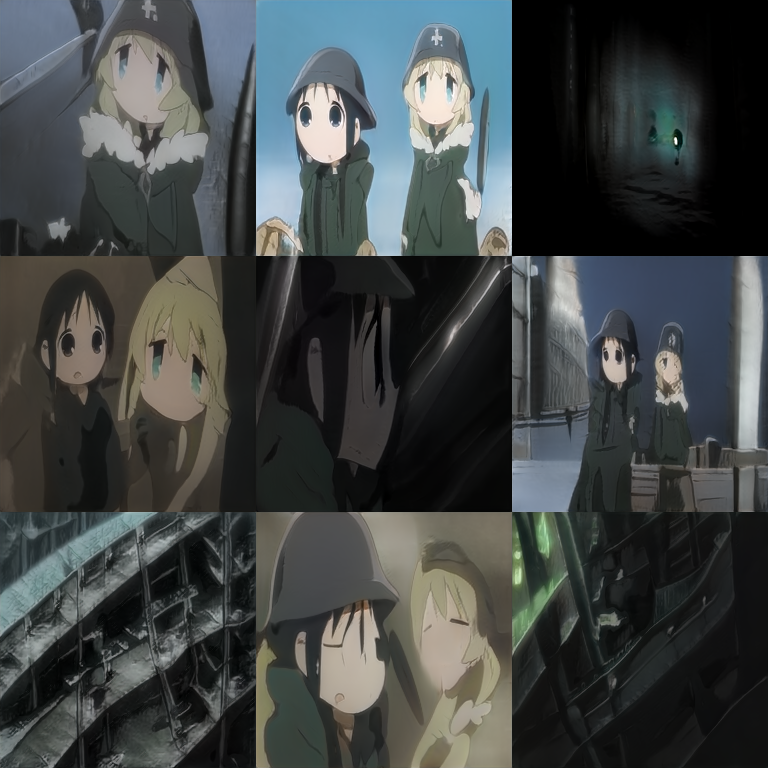
\includegraphics[scale=0.25]{samples_gan}
      \caption{Generated images.}
    \end{subfigure}
    \hfill
    \begin{subfigure}[h]{0.49 \textwidth}
      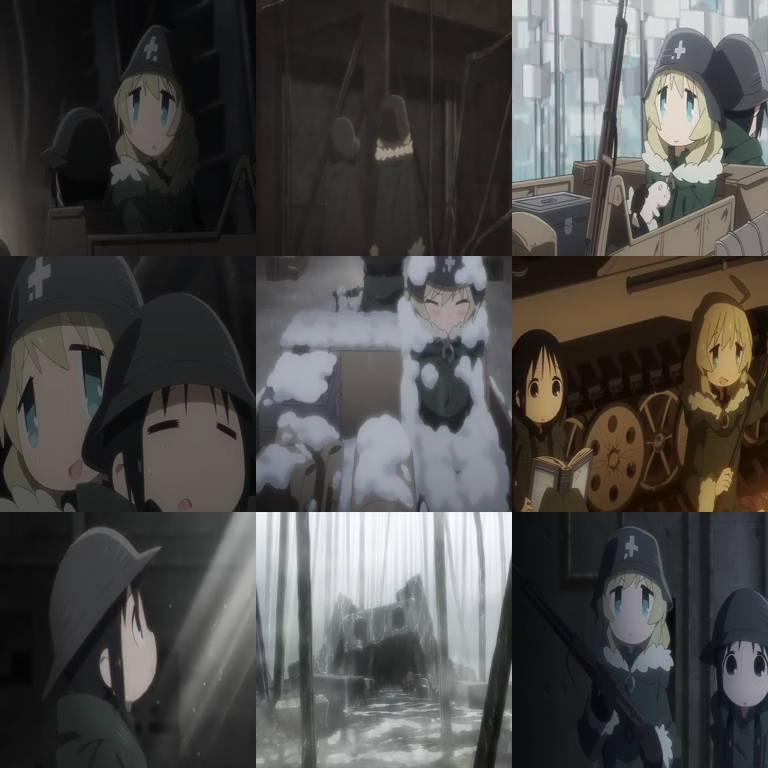
\includegraphics[scale=0.25]{samples_real}
      \caption{Real images.}
    \end{subfigure}
    \caption{Images generated by StyleGAN2-ADA \cite{stylegan2ada} compared to
      ground truth images from \textit{Girls' Last Tour} \cite{tour}. Although
      certain images are strikingly similar (top left of both, middle generated
      image against the bottom left real image), the generated images show
      clear distortions and are discernible from the real images.}
    \label{fig:samples}
\end{figure}

The final model achieves a Fréchet inception distance (FID) of 25.722.
FID is a common metric of generated image quality; we measure FID on 50k
generated images against all training images like \cite{stylegan2ada}. This
is relatively high compared to the FID of 3.88 achieved on the 70k image
FFHQ dataset (human faces) by \cite{stylegan2ada} (lower is better). They
use \( x \)-flips to amplify FFHQ to 140k images, but we also apply \( x
\)-flips to our 170k image dataset so the difference is not of data volume.
We suspect that while the images in FFHQ and similar datasets can be thought
of as independently and identically distributed (i.i.d.) since they are
sampled from the internet, our images are taken from video frames and are
therefore highly correlated with each other. Thus, although we have 170k
images, the diversity of our images is much lower compared to FFHQ which
may explain the poor qualitative results and poor quantitative FID.

\subsection{Conditioning StyleGAN}
We encode an initial frame and its manga page into the latent vector. We
then train our unconditional model to predict successive video frames
with gradient decent given the ground truth video; training details are
described in the appendix, \autoref{app:cond}.

\begin{figure}[h!]
  \centering
  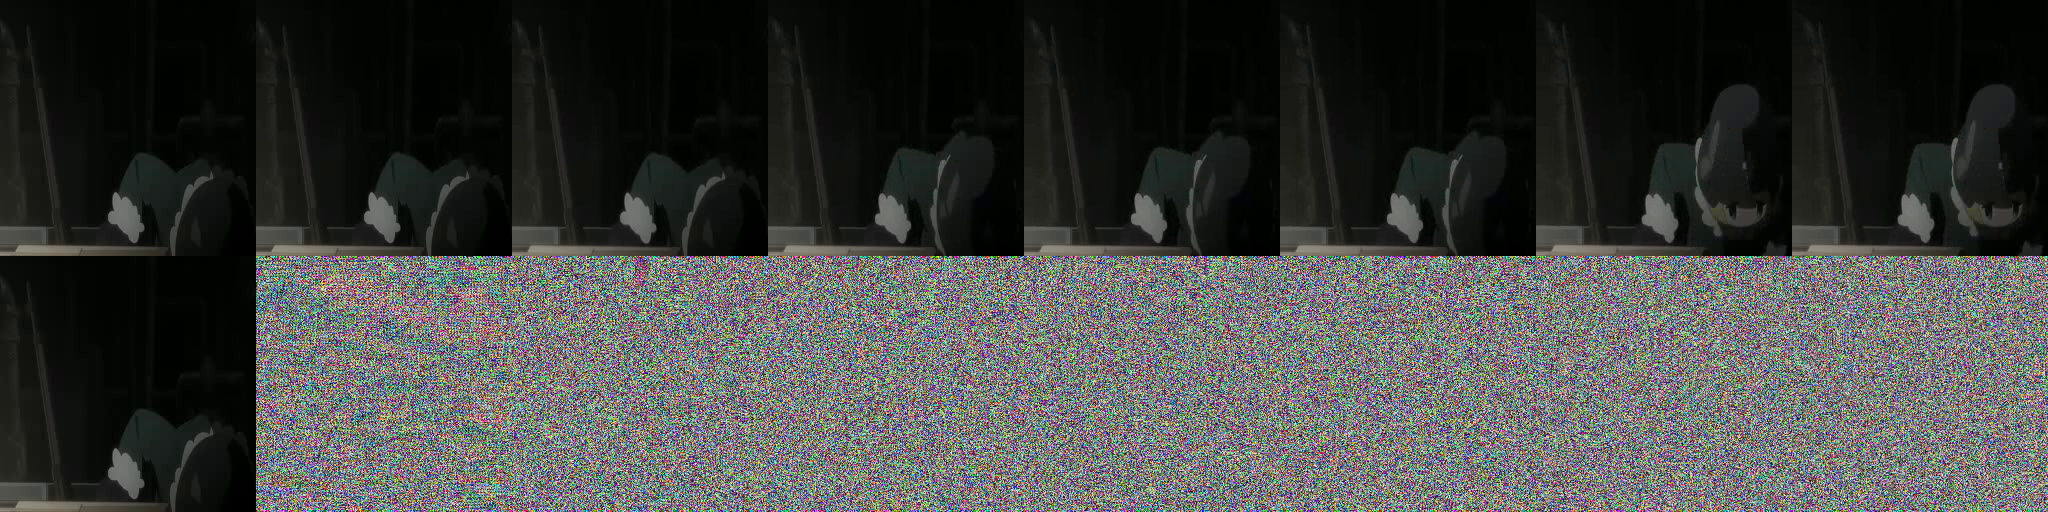
\includegraphics[scale=0.2]{results_gen}
  \caption{StyleGAN2-ADA \cite{stylegan2ada} applied to future video
    prediction with conditioning. Top row is the ground truth 8 frames
    and bottom row is generated output. We notice that the output is
    degenerate noise, which we suspect indicates a capacity issue.}
  \label{fig:gen}
\end{figure}

We find that the generator outputs noise no matter the training duration. We
suspect that this indicates a capacity issue, as \( \bm{z} \)'s dimensionality
of 512 is too small to effectively encode the initial frame and manga page.
As mentioned in \cite{dvdgan}, there is trade-off between unconditional video
synthesis and future video prediction: while future video prediction provides
the ground truth objects and backgrounds which the generator is able to copy
in future frames, helping FID, at the same time the generator is not able
to \enquote{choose} what to generate and must continue what is given. Since
\( \bm{z} \) is not large enough, the generator loses the only benefit of
conditioning and is therefore likely dominated by the discriminator, which
furthermore benefits from conditioning as it has more information.

\subsection{Latent Interpolation}

We first attempt to reconstruct the ground truth video by finding the
corresponding latent vector for each frame. This is shown in the middle row
of \autoref{fig:latent}. We can see that certain frames are reconstructed
well (for example, frames 3, 4, and 7) but other are not represented at all.
We suspect only images frequently occurring can be convincingly represented
by a corresponding latent vector. For linear interpolation, we start from
the frame two seconds into the video and end one second from the end in
order to prevent a completely black generated image. We then linearly
interpolate from the start latent to the end. We find that the resulting
video is perceptually \enquote{smooth}; each frame transitions into the next
without jarring changes. This is to be expected, since the perceptual path
length metric discussed in \cite{stylegan, stylegan2} incentives smooth
transitions. In particular, it directly minimizes the perceptual difference
between adjacent interpolations in the latent space as measured with VGG16
embeddings \cite{stylegan, vgg}. The path length regularization introduced
in \cite{stylegan2} also contributes. Because the shortest path between two
points is a line, a model must map such a path into a shortest path on the
image manifold, or a geodesic \cites{stylegan2}.

\begin{figure}[h!]
  \centering
  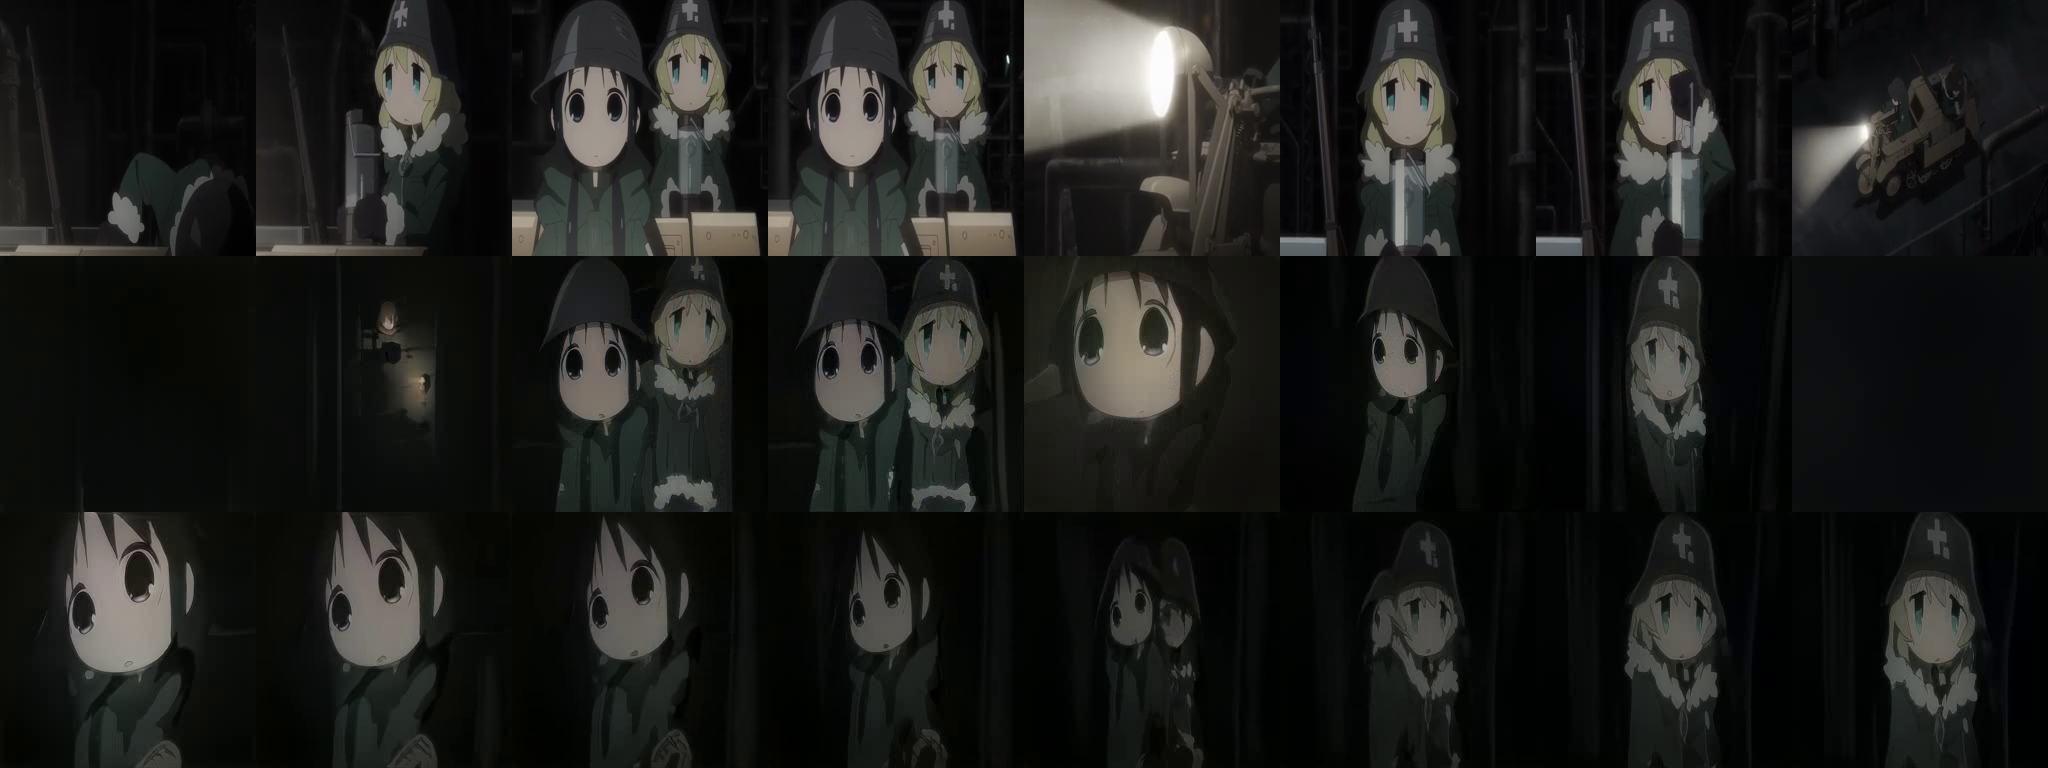
\includegraphics[scale=0.2]{results_latent}
  \caption{StyleGAN2-ADA \cite{stylegan2ada} used for latent interpolation.
    Top row is the ground truth 8 frames sampled evenly over a video with
    duration \( \approx 15 \) seconds, middle row is a reconstruction
    of each frame by finding its corresponding latent vector, and the
    bottom row is a linear interpolation from the start vector to
    the end vector. For the resulting videos and more examples, see
    \href{https://youtu.be/4J9BBHX-uNg}{https://youtu.be/4J9BBHX-uNg}.}
  \label{fig:latent}
\end{figure}

\section{Conclusion}
Dismayed at the state of video generation, we propose the simplified domain
of generating anime. We discuss important features of anime and manga for
efficient generation of a large-scale dataset from unlabeled video on the
internet. We then experiment with adjusting StyleGAN \cite{stylegan2ada} for
future video prediction with conditioning and with linear interpolation in the
latent space. Although our results are poor, we believe the avenues of research
laid out in this work can be improved in future experiments. One possible
approach may be to adjust DVD-GAN \cite{dvdgan} to use a foreground/background
mask \cite{scene} and then upscale the video with a deep super-resolution
algorithm like \href{https://github.com/nagadomi/waifu2x}{waifu2x} or
\href{https://github.com/akai-katto/dandere2x}{dandere2x}.

\paragraph{Acknowledgments}
This project was done in TJHSST's Computer Systems Lab. We thank
Dr. Torbert and Dr. Gabor, our mentors for this research project.

\newpage

\printbibliography

\newpage

\section{Appendix}
\subsection{StyleGAN Training} \label{app:train}
\cite{stylegan2} mentions that the \( R_1 \) parameter \( \gamma
\) significantly depends on the dataset. We experiment with a wide
variety of choices for \( \gamma \) as shown in \autoref{fig:train}.

\begin{figure}[h!]
  \centering
  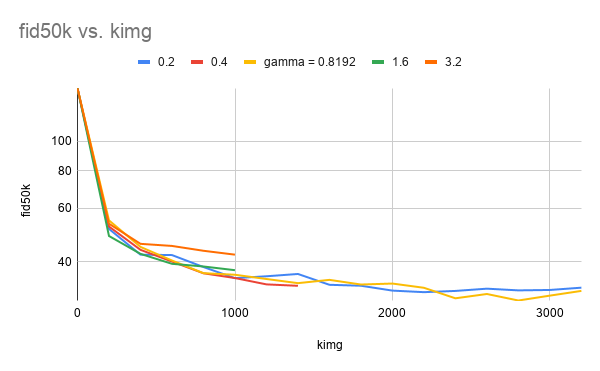
\includegraphics[scale=0.7]{graph}
  \caption{FID over a wide variety of \( \gamma \) choices.}
  \label{fig:train}
\end{figure}

Our final model uses the automatically determined \( \gamma \) of 0.8192
from the resolution of the dataset \cite{stylegan2ada}, \( x \)-flips,
which are shown to improve FID in certain cases \cite{stylegan2ada}, and
transfer learning from a pre-trained model on the FFHQ 256x256 dataset
since transfer learning success seems to depend more on the diversity of
the source dataset rather than the similarity between the two datasets
\cite{stylegan2ada}. After 6200 kimg (thousands of image shown to the
discriminator) the model achieves a FID50k of 25.722, at which point the
FID starts to rise so training was terminated.

\subsection{Conditioning StyleGAN} \label{app:cond}
We use mean squared loss along with the Adam optimizer with
a learning rate of \( \alpha = 0.001 \). We use a batch size
of 16, and ran the model for 4000 batches before stopping.

\end{document}
